\documentclass{article}
\usepackage[utf8x]{inputenc}
\usepackage[T1]{fontenc}
\usepackage{graphicx}
\usepackage{tikz}
\usepackage{pictikzgraph}
\usepackage{float}
\usepackage[left=1cm,right=1cm,top=1cm,bottom=1cm]{geometry}

\begin{document}
\pagenumbering{gobble}
\begin{figure}[H]
 \centering
 
\includegraphics[width=0.5\textwidth]{Pictures/g0.pdf}
 \caption{Input image (\texttt{Pictures/g0.svg}).}
 \end{figure}

 \begin{figure}[H]
 \centering
 \begin{tikzpicture}[scale=1.5]
 \input{Pictures/g0-grid.tex}
 \end{tikzpicture}~
 \begin{tikzpicture}[scale=1.5]
 \input{Pictures/g0-uniform.tex}
 \end{tikzpicture}~
 \begin{tikzpicture}[scale=1.5]
 \input{Pictures/g0-plain.tex}
 \end{tikzpicture}
 \caption{Output of pictikz (grid, uniform, plain)}
 \end{figure}\clearpage

\begin{figure}[H]
 \centering
 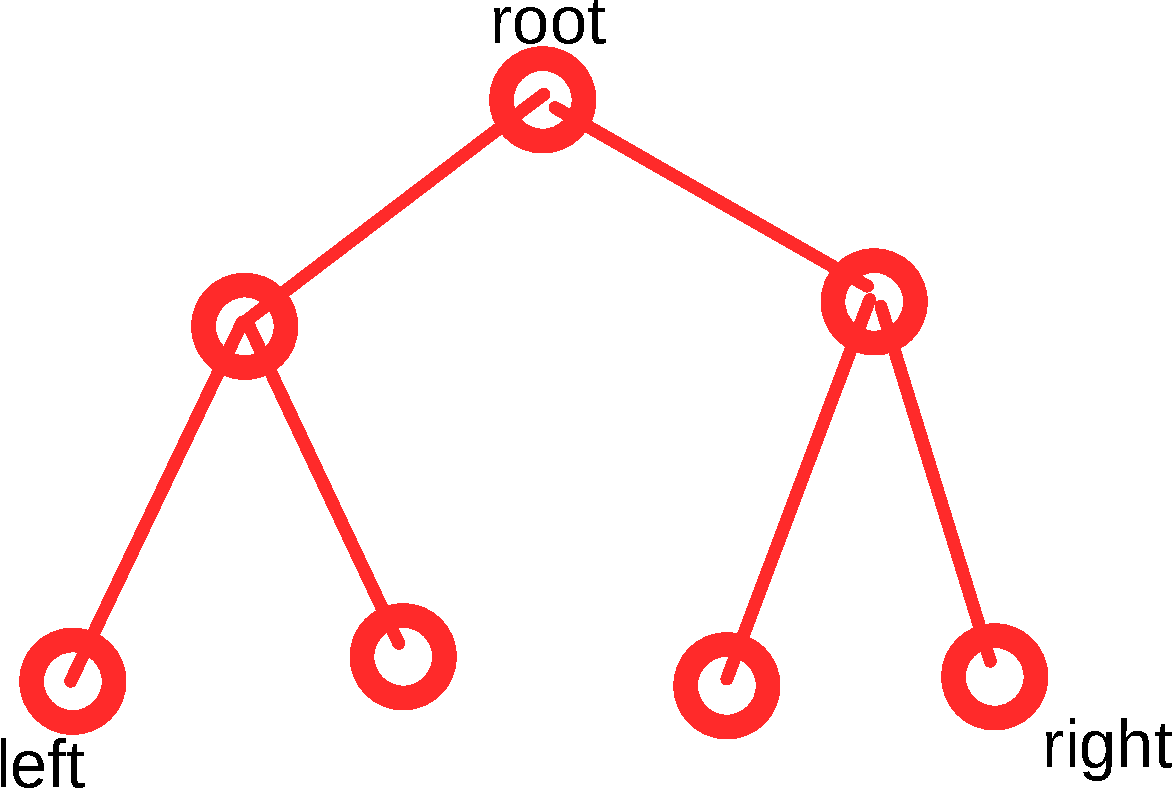
\includegraphics[width=0.5\textwidth]{Pictures/tree.pdf}
 \caption{Input image (\texttt{Pictures/tree.svg}).}
 \end{figure}

 \begin{figure}[H]
 \centering
 \begin{tikzpicture}[scale=1.5]
 \input{Pictures/tree-grid.tex}
 \end{tikzpicture}~
 \begin{tikzpicture}[scale=1.5]
 \input{Pictures/tree-uniform.tex}
 \end{tikzpicture}~
 \begin{tikzpicture}[scale=1.5]
 \input{Pictures/tree-plain.tex}
 \end{tikzpicture}
 \caption{Output of pictikz (grid, uniform, plain)}
 \end{figure}\clearpage

\begin{figure}[H]
 \centering
 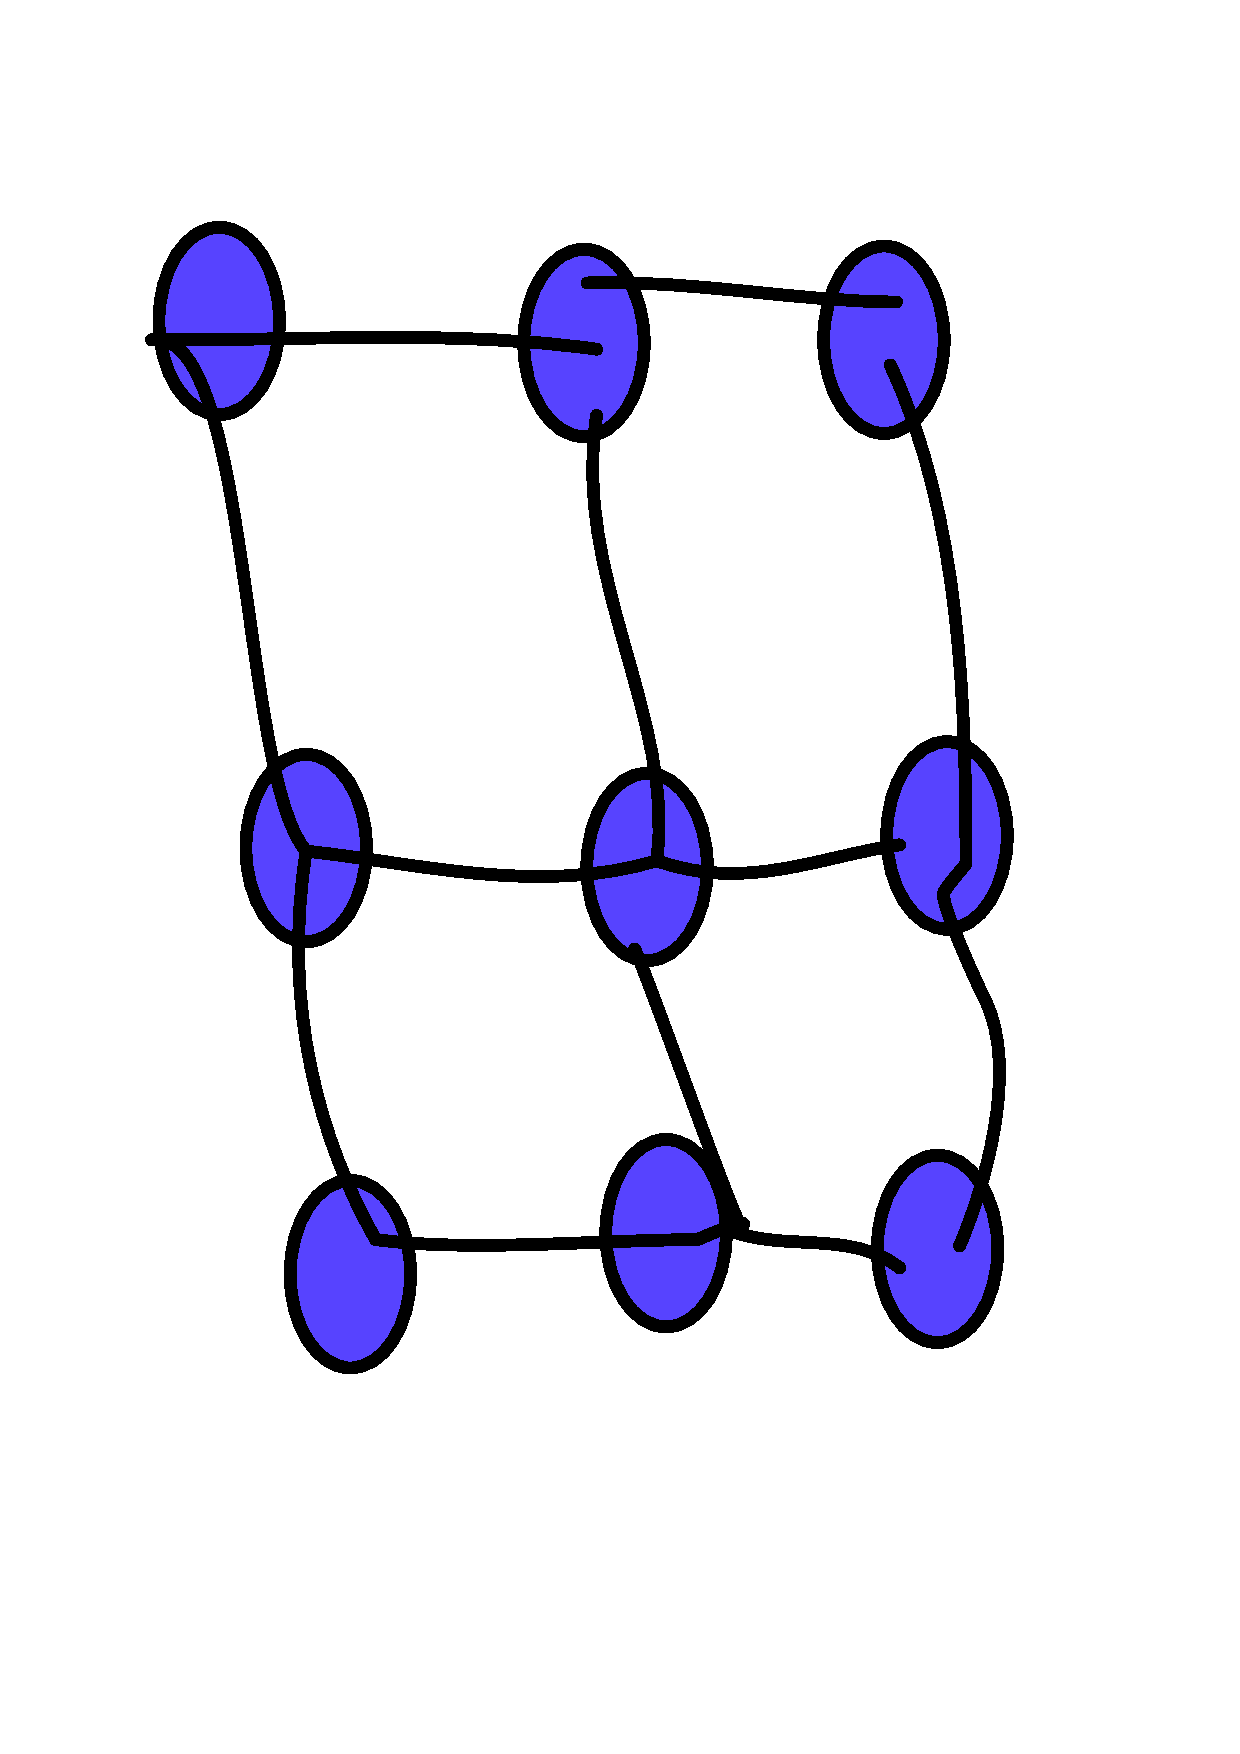
\includegraphics[width=0.5\textwidth]{Pictures/grid.pdf}
 \caption{Input image (\texttt{Pictures/grid.svg}).}
 \end{figure}

 \begin{figure}[H]
 \centering
 \begin{tikzpicture}[scale=1.5]
 \input{Pictures/grid-grid.tex}
 \end{tikzpicture}~
 \begin{tikzpicture}[scale=1.5]
 \input{Pictures/grid-uniform.tex}
 \end{tikzpicture}~
 \begin{tikzpicture}[scale=1.5]
 \input{Pictures/grid-plain.tex}
 \end{tikzpicture}
 \caption{Output of pictikz (grid, uniform, plain)}
 \end{figure}\clearpage

\begin{figure}[H]
 \centering
 
\includegraphics[width=0.5\textwidth]{Pictures/network-a.pdf}
 \caption{Input image (\texttt{Pictures/network-a.svg}).}
 \end{figure}

 \begin{figure}[H]
 \centering
 \begin{tikzpicture}[scale=1.5]
 \input{Pictures/network-a-grid.tex}
 \end{tikzpicture}~
 \begin{tikzpicture}[scale=1.5]
 \input{Pictures/network-a-uniform.tex}
 \end{tikzpicture}~
 \begin{tikzpicture}[scale=1.5]
 \input{Pictures/network-a-plain.tex}
 \end{tikzpicture}
 \caption{Output of pictikz (grid, uniform, plain)}
 \end{figure}\clearpage

\begin{figure}[H]
 \centering
 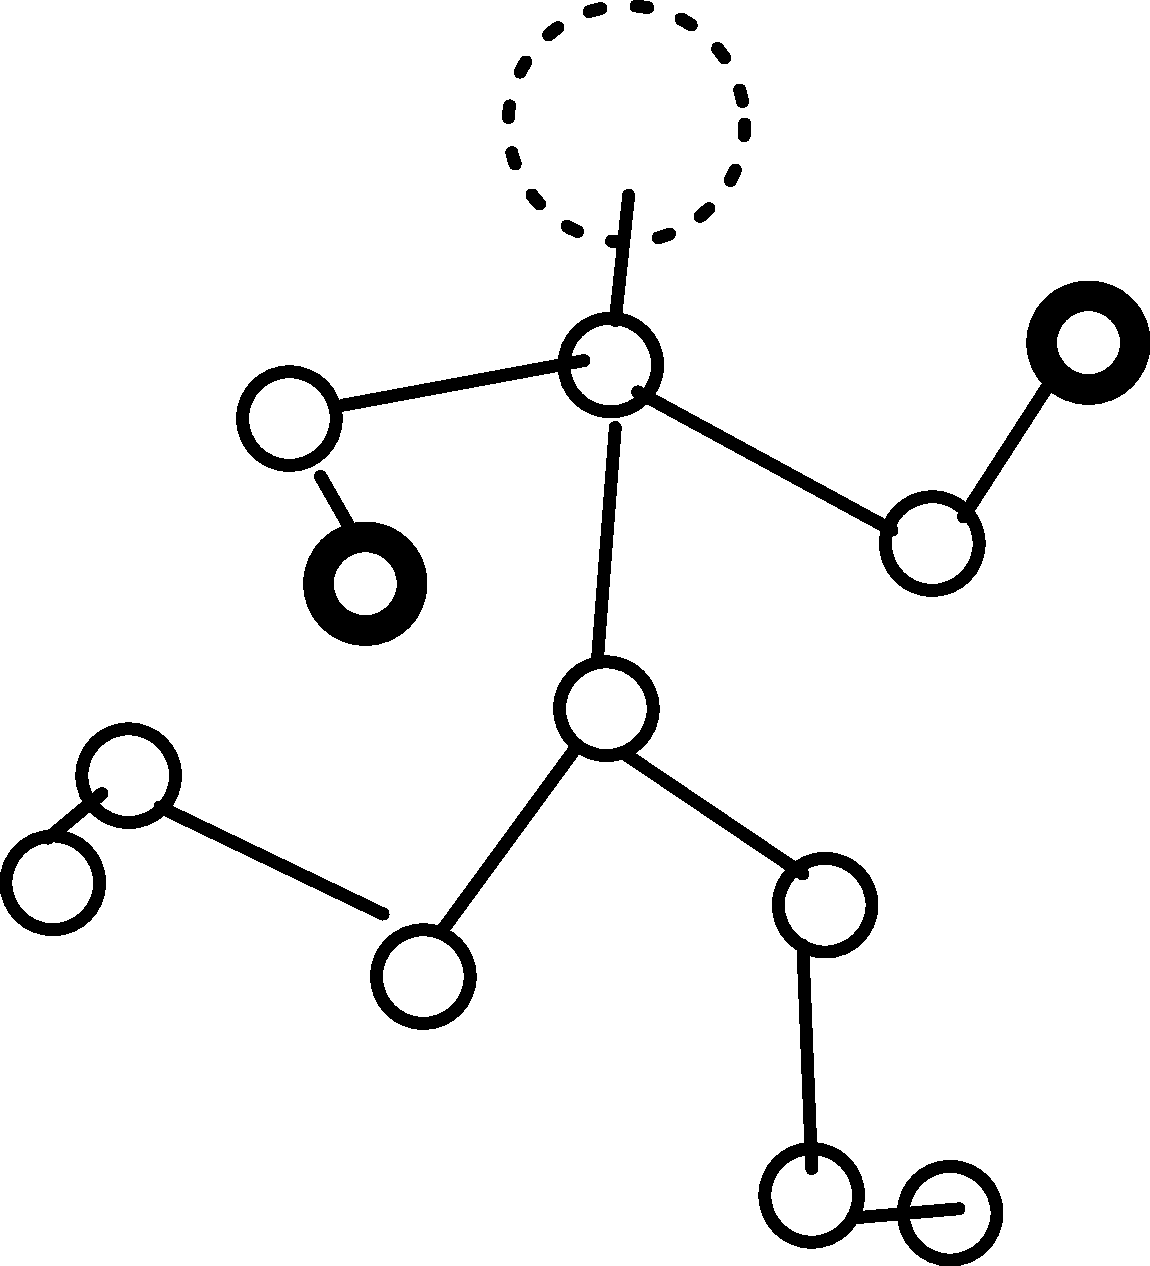
\includegraphics[width=0.5\textwidth]{Pictures/running-man.pdf}
 \caption{Input image (\texttt{Pictures/running-man.svg}).}
 \end{figure}

 \begin{figure}[H]
 \centering
 \begin{tikzpicture}[scale=1.5]
 \input{Pictures/running-man-grid.tex}
 \end{tikzpicture}~
 \begin{tikzpicture}[scale=1.5]
 \input{Pictures/running-man-uniform.tex}
 \end{tikzpicture}~
 \begin{tikzpicture}[scale=1.5]
 \input{Pictures/running-man-plain.tex}
 \end{tikzpicture}
 \caption{Output of pictikz (grid, uniform, plain)}
 \end{figure}\clearpage

\begin{figure}[H]
 \centering
 
\includegraphics[width=0.5\textwidth]{Pictures/rotation.pdf}
 \caption{Input image (\texttt{Pictures/rotation.svg}).}
 \end{figure}

 \begin{figure}[H]
 \centering
 \begin{tikzpicture}[scale=1.5]
 \input{Pictures/rotation-grid.tex}
 \end{tikzpicture}~
 \begin{tikzpicture}[scale=1.5]
 \input{Pictures/rotation-uniform.tex}
 \end{tikzpicture}~
 \begin{tikzpicture}[scale=1.5]
 \input{Pictures/rotation-plain.tex}
 \end{tikzpicture}
 \caption{Output of pictikz (grid, uniform, plain)}
 \end{figure}\clearpage

\begin{figure}[H]
 \centering
 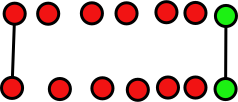
\includegraphics[width=0.5\textwidth]{Pictures/long-grid.pdf}
 \caption{Input image (\texttt{Pictures/long-grid.svg}).}
 \end{figure}

 \begin{figure}[H]
 \centering
 \begin{tikzpicture}[scale=1.5]
 \input{Pictures/long-grid-grid.tex}
 \end{tikzpicture}~
 \begin{tikzpicture}[scale=1.5]
 \input{Pictures/long-grid-uniform.tex}
 \end{tikzpicture}~
 \begin{tikzpicture}[scale=1.5]
 \input{Pictures/long-grid-plain.tex}
 \end{tikzpicture}
 \caption{Output of pictikz (grid, uniform, plain)}
 \end{figure}\clearpage

\begin{figure}[H]
 \centering
 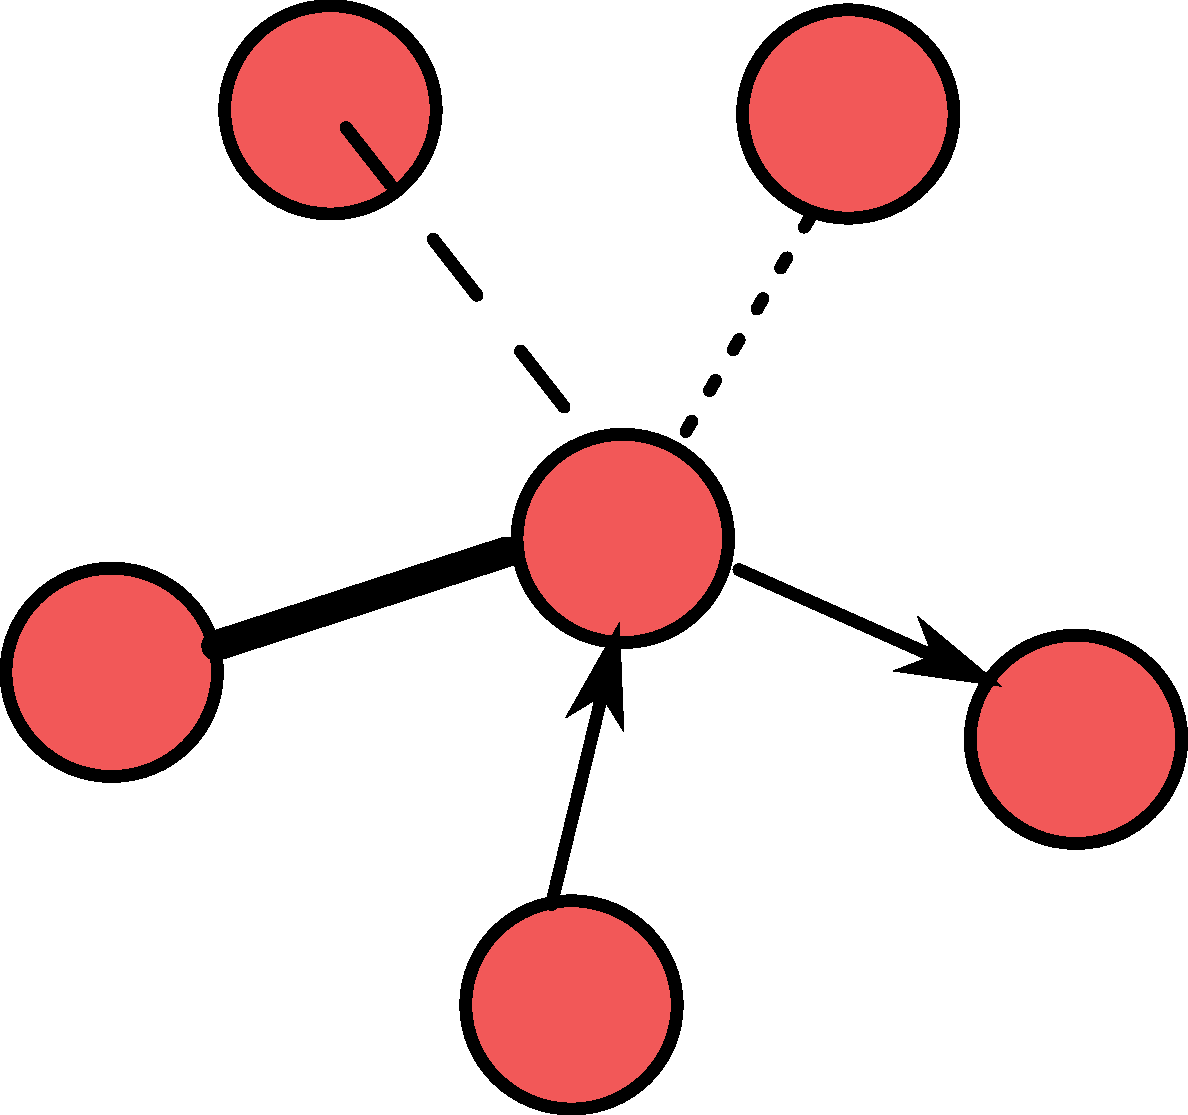
\includegraphics[width=0.5\textwidth]{Pictures/star.pdf}
 \caption{Input image (\texttt{Pictures/star.svg}).}
 \end{figure}

 \begin{figure}[H]
 \centering
 \begin{tikzpicture}[scale=1.5]
 \input{Pictures/star-grid.tex}
 \end{tikzpicture}~
 \begin{tikzpicture}[scale=1.5]
 \input{Pictures/star-uniform.tex}
 \end{tikzpicture}~
 \begin{tikzpicture}[scale=1.5]
 \input{Pictures/star-plain.tex}
 \end{tikzpicture}
 \caption{Output of pictikz (grid, uniform, plain)}
 \end{figure}\clearpage

\begin{figure}[H]
 \centering
 
\includegraphics[width=0.5\textwidth]{Pictures/marketing.pdf}
 \caption{Input image (\texttt{Pictures/marketing.svg}).}
 \end{figure}

 \begin{figure}[H]
 \centering
 \begin{tikzpicture}[scale=1.5]
 \input{Pictures/marketing-grid.tex}
 \end{tikzpicture}~
 \begin{tikzpicture}[scale=1.5]
 \input{Pictures/marketing-uniform.tex}
 \end{tikzpicture}~
 \begin{tikzpicture}[scale=1.5]
 \input{Pictures/marketing-plain.tex}
 \end{tikzpicture}
 \caption{Output of pictikz (grid, uniform, plain)}
 \end{figure}\clearpage

\begin{figure}[H]
 \centering
 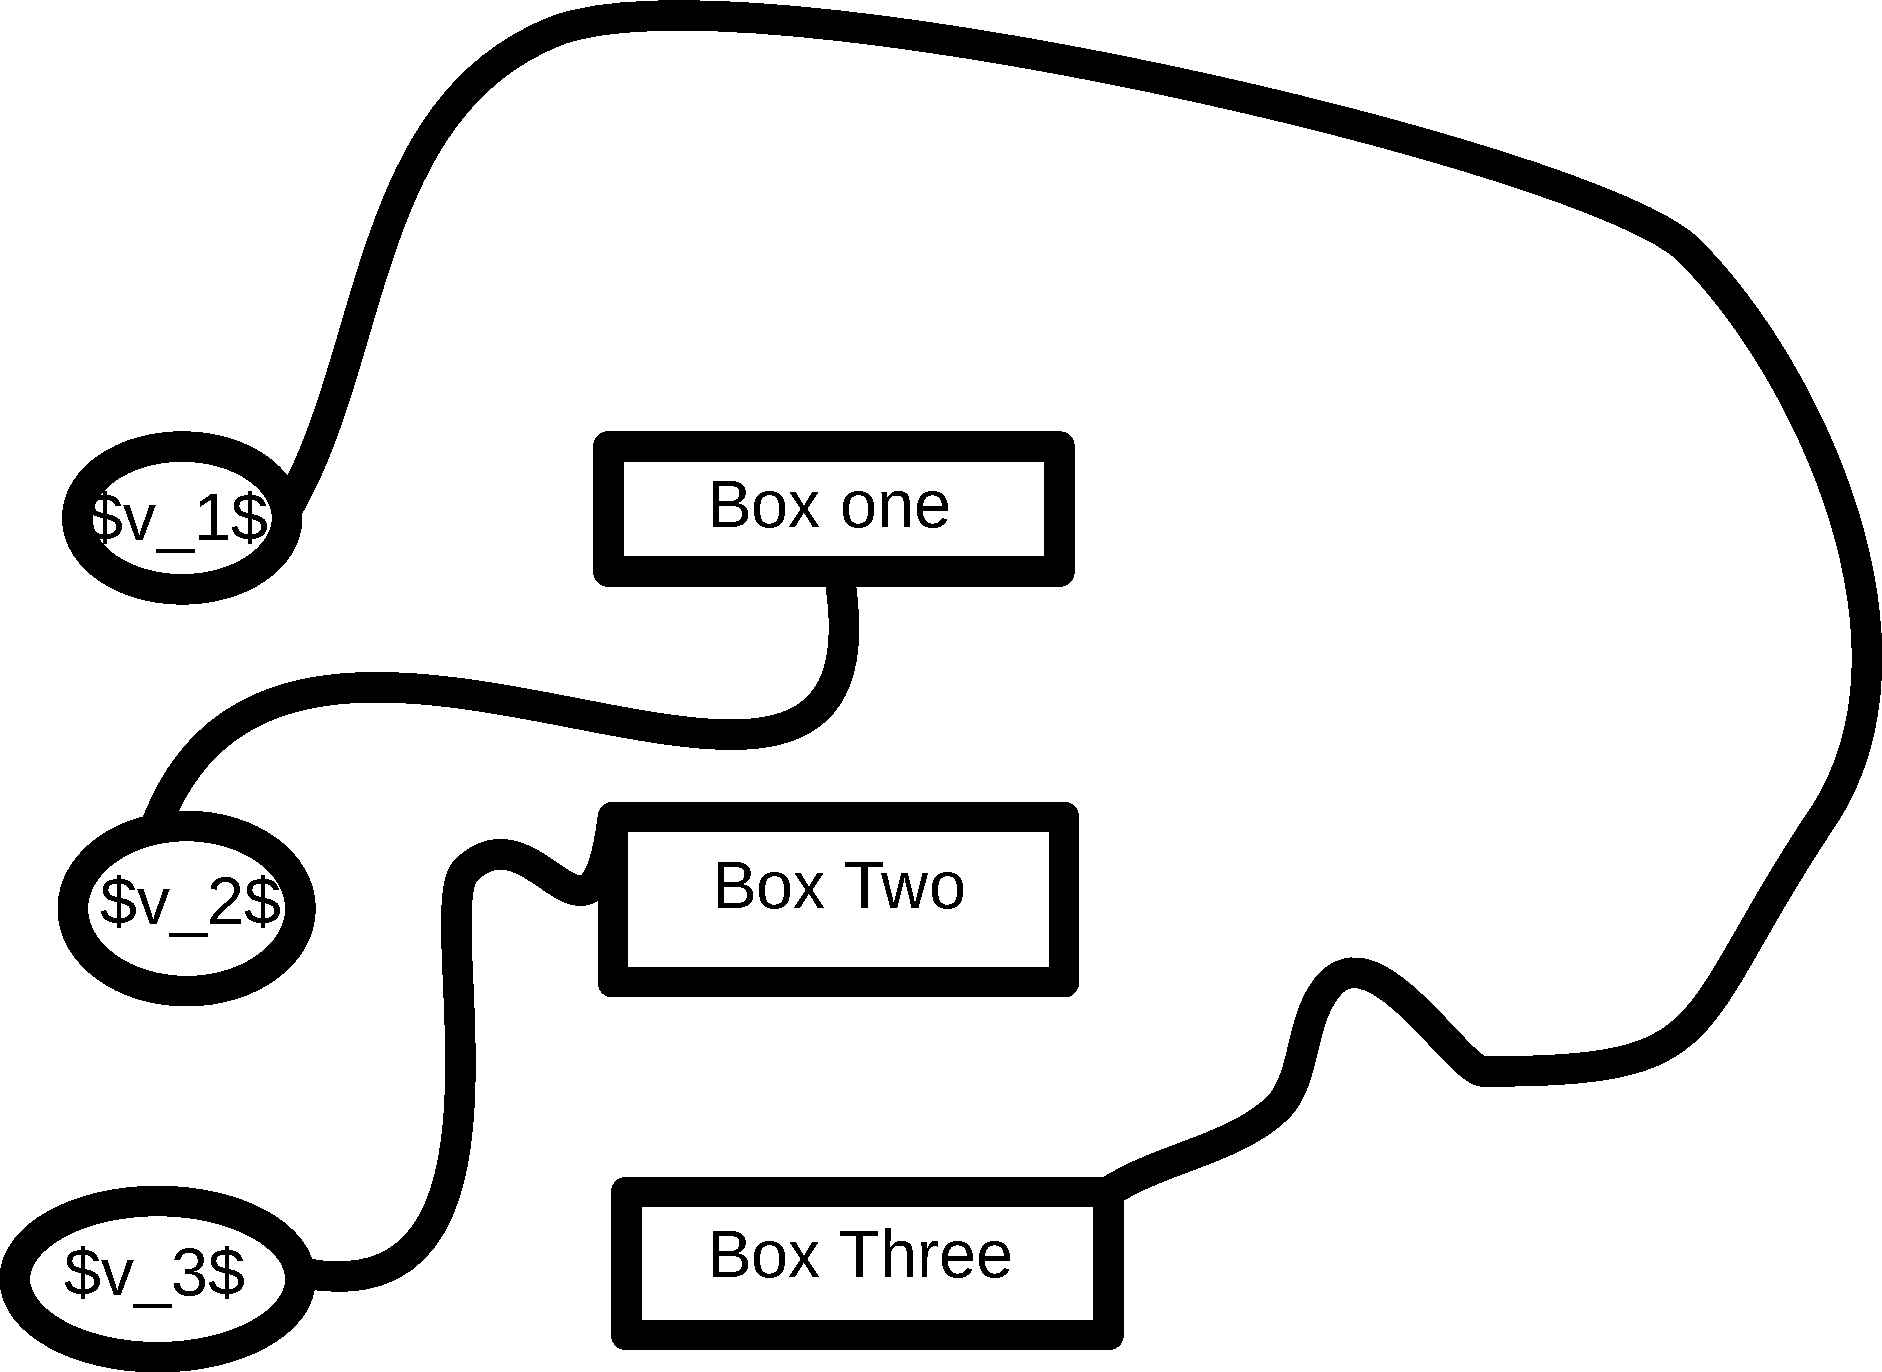
\includegraphics[width=0.5\textwidth]{Pictures/box.pdf}
 \caption{Input image (\texttt{Pictures/box.svg}).}
 \end{figure}

 \begin{figure}[H]
 \centering
 \begin{tikzpicture}[scale=1.5]
 \input{Pictures/box-grid.tex}
 \end{tikzpicture}~
 \begin{tikzpicture}[scale=1.5]
 \input{Pictures/box-uniform.tex}
 \end{tikzpicture}~
 \begin{tikzpicture}[scale=1.5]
 \input{Pictures/box-plain.tex}
 \end{tikzpicture}
 \caption{Output of pictikz (grid, uniform, plain)}
 \end{figure}\clearpage

\begin{figure}[H]
 \centering
 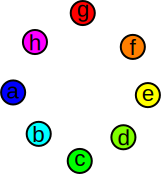
\includegraphics[width=0.5\textwidth]{Pictures/color-wheel.pdf}
 \caption{Input image (\texttt{Pictures/color-wheel.svg}).}
 \end{figure}

 \begin{figure}[H]
 \centering
 \begin{tikzpicture}[scale=1.5]
 \input{Pictures/color-wheel-grid.tex}
 \end{tikzpicture}~
 \begin{tikzpicture}[scale=1.5]
 \input{Pictures/color-wheel-uniform.tex}
 \end{tikzpicture}~
 \begin{tikzpicture}[scale=1.5]
 \input{Pictures/color-wheel-plain.tex}
 \end{tikzpicture}
 \caption{Output of pictikz (grid, uniform, plain)}
 \end{figure}\clearpage

\begin{figure}[H]
 \centering
 
\includegraphics[width=0.5\textwidth]{Pictures/styled-text.pdf}
 \caption{Input image (\texttt{Pictures/styled-text.svg}).}
 \end{figure}

 \begin{figure}[H]
 \centering
 \begin{tikzpicture}[scale=1.5]
 \input{Pictures/styled-text-grid.tex}
 \end{tikzpicture}~
 \begin{tikzpicture}[scale=1.5]
 \input{Pictures/styled-text-uniform.tex}
 \end{tikzpicture}~
 \begin{tikzpicture}[scale=1.5]
 \input{Pictures/styled-text-plain.tex}
 \end{tikzpicture}
 \caption{Output of pictikz (grid, uniform, plain)}
 \end{figure}\clearpage

\begin{figure}[H]
 \centering
 
\includegraphics[width=0.5\textwidth]{Pictures/text-circle.pdf}
 \caption{Input image (\texttt{Pictures/text-circle.svg}).}
 \end{figure}

 \begin{figure}[H]
 \centering
 \begin{tikzpicture}[scale=1.5]
 \input{Pictures/text-circle-grid.tex}
 \end{tikzpicture}~
 \begin{tikzpicture}[scale=1.5]
 \input{Pictures/text-circle-uniform.tex}
 \end{tikzpicture}~
 \begin{tikzpicture}[scale=1.5]
 \input{Pictures/text-circle-plain.tex}
 \end{tikzpicture}
 \caption{Output of pictikz (grid, uniform, plain)}
 \end{figure}\clearpage

\end{document}
